\documentclass[convert={svg,command=\unexpanded{{inkscape\space --pdf-poppler\space --export-type="svg"\space --pages=1\space -o\space \outfile\space \infile}}}]{standalone}% 'crop' is the default for v1.0, before it was 'preview'

\usepackage{tikz}
\usepackage{pgfplots}
\usepgfplotslibrary{fillbetween}
\usetikzlibrary{patterns, patterns.meta, positioning, math}

\pgfplotsset{compat=1.18}

\usepackage{tikz-3dplot}
\usetikzlibrary{3d,calc}

\pgfplotsset{
	twoDaxis/.style = {
			no marks,
			samples = 100,
			axis lines = center,
			xlabel = {$x$},
			ylabel = {$y$},
			every axis x label/.style={
					at={(ticklabel* cs:1.05)},
					anchor=west,
				},
			every axis y label/.style={
					at={(ticklabel* cs:1.05)},
					anchor=south,
				},
		},
	threeDaxis/.style = {
			axis z line = none,
			axis lines=center, % remove this and you get weird box behavior, not good for calc 2 students
			xlabel=$x$, % you know this one
			every axis x label/.style={
					at={(ticklabel* cs:1.05)},
					anchor=west,
				}, % place the xlabel in a better spot
			ylabel=$y$, % you know this one
			every axis y label/.style={
					at={(ticklabel* cs:1.05)},
					anchor=north,
				}, % places y label in a better spot
		},
	threeDaxiswithyzswap/.style = {
			axis y line = none,
			axis lines=center, % remove this and you get weird box behavior, not good for calc 2 students
			xlabel=$x$, % you know this one
			every axis x label/.style={
					at={(ticklabel* cs:1.05)},
					anchor=west,
				}, % place the xlabel in a better spot
			zlabel=$y$, % you know this one
			every axis z label/.style={
					at={(ticklabel* cs:1.05)},
					anchor=south, % which side of the label gets pinned to the point 5% past the axis end point?
				}, % places y label in a better spot
			xticklabel style = {font=\tiny, yshift=1ex},
			zticklabel style = {font=\tiny, xshift=1ex},
		}
}

\def\centerarc[#1](#2)(#3:#4:#5)% Syntax: [draw options] (center) (initial angle:final angle:radius)
{ \draw[#1] ($(#2)+(axis direction cs:{#5*cos(#3)},{#5*sin(#3)})$) arc (#3:#4:#5); }

\def\centerarc[#1](#2)(#3:#4:#5:#6)% Syntax: [draw options] (center) (initial angle:final angle:xradius:yradius)
{ \draw[#1] ($(#2)+(axis direction cs:{#5*cos(#3)},{#6*sin(#3)})$) arc  [start angle = #3, end angle = #4, x radius = #5, y radius = #6]; }

\def\diskslicevert[#1](#2)(#3:#4)% Syntax: [draw options] (center) (xradius:yradius) use {} if functions on things!!!!!!
{ 		\draw [<->, #1] (#2) -- ($(#2)+(axis direction cs:{0},{#4})$) node [midway, right] {$R$};
	\centerarc[#1](#2)(20:340:{#3}:{#4});
	\centerarc[dotted, #1](#2)(340:380:{#3}:{#4});
}
\def\diskslicevert[#1,r=#2](#3)(#4:#5)% Syntax: [draw options] (center) (xradius:yradius)
{ 		\draw [<->, #1] (#3) -- ($(#3)+(axis direction cs:{0},{#5})$) node [midway, right] {#2};
	\centerarc[#1](#3)(20:340:{#4}:{#5});
	\centerarc[dotted, #1](#3)(340:380:{#4}:{#5});
}
\def\diskslicevertflip[#1,r=#2](#3)(#4:#5)% Syntax: [draw options] (center) (xradius:yradius)
{ 		\draw [<->, #1] (#3) -- ($(#3)+(axis direction cs:{0},{-#5})$) node [midway, right] {#2};
	\centerarc[#1](#3)(20:340:{#4}:{#5});
	\centerarc[dotted, #1](#3)(340:380:{#4}:{#5});
}
\def\diskslicehor[#1](#2)(#3:#4)% Syntax: [draw options] (center) (xradius:yradius)
{ 	\draw [<->, #1] (#2) -- ($(#2)+(axis direction cs:{#3},{0})$) node [midway, above] {$R$};
	\centerarc[#1](#2)(0:70:#3:#4);
	\centerarc[dotted, #1](#2)(70:110:#3:#4);
	\centerarc[#1](#2)(110:360:#3:#4);
}
\def\diskslicehor[#1,r=#2](#3)(#4:#5)% Syntax: [draw options] (center) (xradius:yradius)
{ 	\draw [<->, #1] (#3) -- ($(#3)+(axis direction cs:{#4},{0})$) node [midway, above] {#2};
	\centerarc[#1](#3)(0:70:#4:#5);
	\centerarc[dotted, #1](#3)(70:110:#4:#5);
	\centerarc[#1](#3)(110:360:#4:#5);
}
\def\diskslicehorflip[#1,r=#2](#3)(#4:#5)% Syntax: [draw options] (center) (xradius:yradius)
{ 	\draw [<->, #1] (#3) -- ($(#3)+(axis direction cs:{-#4},{0})$) node [midway, above] {#2};
	\centerarc[#1](#3)(0:70:#4:#5);
	\centerarc[dotted, #1](#3)(70:110:#4:#5);
	\centerarc[#1](#3)(110:360:#4:#5);
}

\usetikzlibrary{decorations.text, decorations.pathmorphing, topaths} 


\begin{document}
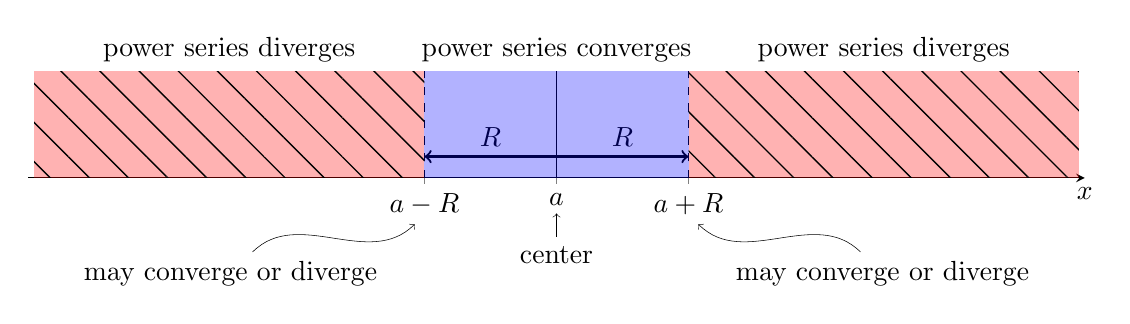
\begin{tikzpicture}
	\begin{axis}[
			twoDaxis,
			axis y line = none,
			ymin = -1,
			ymax = 1,
			xmin = -16,
			xmax = 20,
			xtick = {-2.5,2,6.5},
			xticklabels = {$a-R$,$a$,$a+R$},
			% xlabel = {$x$},
			width = 15cm,
			height = 7cm,
			every axis x label/.style={
					at={(ticklabel* cs:1.)},
					anchor=north,
				},
		]
		\addplot[->,thick] (2,.1) -- (6.5,.1) node[midway, above] {$R$};
		\addplot[->,thick] (2,.1) -- (-2.5,.1) node[midway, above] {$R$};

		\addplot[black] (2,0) -- (2,0.5) node[at end, above] {power series converges} node[pos=-0.15,below,pin={[pin distance=.3cm, pin edge={<-,black, out=270, in=90}]below :center}] {};
		\addplot[dashed] (-2.5,0) -- (-2.5,0.5) node[pos=-0.25,below,pin={[pin distance=.5cm, pin edge={<-,black, out=225, in=45,solid}]below left:may converge or diverge}] {};
		\addplot[dashed] (6.5,0) -- (6.5,0.5) node[pos=-0.25,below,pin={[pin distance=.5cm, pin edge={<-,black, out=-45, in=135,solid}]below right:may converge or diverge}] {};

		\fill[fill opacity=0.3,	draw=none,	fill=blue,] (6.5,0) -- (6.5,0.5) -- (-2.5,0.5) -- (-2.5,0) -- cycle;
		\fill[fill opacity=0.3,	draw=none,	fill=red,] (6.5,0) -- (6.5,0.5) -- node[midway, above, opacity=1] {power series diverges} (19.8,0.5) -- (19.8,0) -- cycle;
		\fill[fill opacity=0.3,	draw=none,	fill=red,] (-15.8,0) -- (-15.8,0.5) -- node[midway, above, opacity=1] {power series diverges} (-2.5,0.5) -- (-2.5,0) -- cycle;

		\fill[fill opacity=0.3,	draw=none, pattern = {Lines[angle=135,distance=10pt,line width=.5pt]}] (6.5,0) -- (6.5,0.5) -- (19.8,0.5) -- (19.8,0) -- cycle;
		\fill[fill opacity=0.3,	draw=none, pattern = {Lines[angle=135,distance=10pt,line width=.5pt]}] (-15.8,0) -- (-15.8,0.5) -- (-2.5,0.5) -- (-2.5,0) -- cycle;

	\end{axis}
\end{tikzpicture}
\end{document}